
% File eamt15.tex, an adaptation of eamt14.tex (which was a copy of
% eamt12.tex)
%
% Contact: eamt2015@dlsi.ua.es

%%% To ease future customizations, various replaceables have been paramaterized
%%% as listed in the newcommands section

\documentclass[11pt]{article}
\usepackage{eamt15}
\usepackage{times}
\usepackage{latexsym}
\setlength\titlebox{6.5cm}    % Expanding the titlebox
%%% YOUR PACKAGES BELOW THIS LINE %%%
\usepackage{url}

\usepackage{multirow}


\usepackage{polyglossia}
\setdefaultlanguage[variant=australian]{english}
\usepackage{latexsym}
%\usepackage[small,bf]{caption}
\usepackage[bf]{caption}
\usepackage{xltxtra}
\usepackage{times}
\usepackage{fontspec}
\defaultfontfeatures{Scale=MatchLowercase,Mapping=tex-text}
\usepackage{listings}

\newfontfeature{IPA}{+mgrk}
%\setromanfont[IPA]{FreeSerif}
%\setromanfont[Scale=0.9]{Times New Roman}
\setromanfont{Times New Roman}
\newfontfamily\qipa[IPA,Scale=MatchLowercase]{FreeSerif}
\newfontfamily\qipb[IPA,Scale=MatchLowercase]{Junicode}
\setmonofont[Scale=0.7]{DejaVu Sans Mono}
\newfontfamily\smallertt[Scale=0.55]{DejaVu Sans Mono}
\newfontfamily\smallerrm[Scale=0.85]{Times New Roman}

%\fontspec[FakeBold=2.5]{Times New Roman}
%\DeclareFontShape{EU1}{TimesNewRoman(0)}{m}{sc}{<->ssub * TimesNewRoman(1)/m/sc}{}



\newcommand{\confname}{EAMT 2015}
\newcommand{\website}{http://www.eamt2015.org/}
\newcommand{\contactname}{the conference chairs (Felipe
  S\'anchez-Mart\'inez, Gema Ram\'irez-S\'anchez and Fred Hollowood)}
\newcommand{\contactemail}{eamt2015@dlsi.ua.es}
\newcommand{\conffilename}{eamt15}
\newcommand{\downloadsite}{http://www.eamt2015.org/}
\newcommand{\paperlength}{$8$ (eight)}
\newcommand{\shortpaperlength}{$4$ (four)}

\newcommand{\com}[1]{\marginpar{\scriptsize #1}} 

\title{A free/open-source machine translation system for English to Kazakh}

% Authors:
% Aida, Mikel, Fran, Inari, ... ?

\date{}

\begin{document}
\maketitle 

\begin{abstract}
..
\end{abstract}

\section{Introduction}

This paper presents a shallow-transfer rule-based machine translation system from English into Kazakh language. First of all, English language is a West Germanic language and Kazakh belong to group of Turkic languages. Therefore, the complex agglutinative morphology of Kazakh language is very different from morphologically not too complex language like English; on the other hand, Turkic language morphology shows clear morphotactics (ordering of morphemes), its morphophonology shows complex phonological changes to due to interactions between neighboring morphemes (vowel harmony, sonorization, etc.) many of which are explicitly represented in writing.
On the other hand, there are many differences between the syntax of Turkic languages and English:.subject-adverb–object–verb order (compare subject–verb–object-adverb in English), use of postpositions (compare prepositions in English), head-final syntax with modifiers and specifiers always preceding the modified/specified (normally following in English), overt case marking allowing for a rather free ordering of arguments (versus a more fixed order in English), lack of definite articles (extensively used in English), verbal-noun-centered structures where English uses modal verbs (must, have to, want to) or verbal-noun or verbal-adjective-centered constructions where English has subordinate clauses using finite verbs with relatives or subordinating conjunctions (the book which I read, the place where I saw him, before he came), lack of a parallel of the English verb have, as used for possession, etc. For an account (in Russian) of syntax differences between English and Kazakh, see Печерских \& Амангельдина (2012).
This paper describes work in progress of development of machine translation system for English-to-Kazakh, which developed by using Apertium free/open-source machine translation platform (Forcada et al. 2011, http://www.apertium.org). 

\section{The Apertium platform}
Apertium (Forcada et al. 2011, http://www.apertium.org) is a free/open-source rule-based machine translation (MT) platform that was built in 2005 by the Universitat d’Alacant. At first, it was initially aimed to translate texts between closely related languages, then it was extended to deal with unrelated languages. This platform has next components: machine translation engine, developer’s tools, and linguistic data for an increasing number of language pairs and they are licensed under the free/open-source GNU General Public License (GPL, versions 2 and 3).

\begin{figure*}[htbp]
\begin{center}
 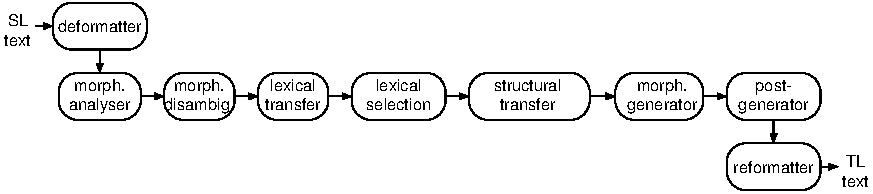
\includegraphics[width=0.8\textwidth]{architecture.pdf}
\end{center}
\caption{The pipeline architecture of the Apertium system.}
\label{fig:modules}
%\vspace{-1em}
\end{figure*}

\begin{itemize}
\item 	De-formatter. Separates the text to be translated from the formatting tags.  Formatting tags are encapsulated in brackets so they are treated as “superblanks” that are placed between words in such a way that the remaining modules see them as regular blanks.  
\item	Morphological analyser. For each surface form the morphological analyser generates one or more lexical forms, which consist of: lemma (dictionary or citation form), lexical category (or part-of-speech), and inflection information. 
For example, the morphological analyser will deliver next sentence "I played" as showed below:
\begin{verbatim}
^I/I<prn><subj><p1><mf><sg>$ 
^played/play<vblex><past>/play<vblex><pp>$
\end{verbatim}
In this example each source form has been analysed as one or more lexical forms: "I" is analysed into "I", where lexical category is subject pronoun(<prn><subj>) and first person(p1), could be masculine or feminine(mf), singular(sg); "played" is analysed into lexical verb(vblex) "play" with past simple tense(past) or it could be past participle(pp), so it has two analysis. Each analysis of word are separated by \texttt{\^{}} and \texttt{\$} symbols, and for one word each lexical forms are delimited by "/", and tags(<...>) show grammatical attributes of lexical form. 
 For Kazakh language finite state transducer based on two-level rules (in the case of Kazakh, apertium-kaz.kaz.lexc, apertium-kaz.kaz.twol). This module therefore separates lexemes and processes morphological analysis, and then returns possible lexical forms.
\item	Part-of-speech (POS) tagger. This module chooses one of lexical forms of ambiguous word. As can be seen from the previous example, the morphological analyser could deliver more than one lexical form and choosing wrong one could produce errors in translation. POS tagger is based on a statistical model, which based on hidden Markov models and it has been trained on source language texts, which processes the result of the application of  on constraint-grammar rules (Karlsson 2005), which areused to discard some analyses  using simple rules (written in apertium-eng-kaz.eng-kaz.rlx) based on context. For example, consider the morphological analysis of word "book":
\begin{verbatim}
^book/book<n><sg>
/book<vblex><inf>
/book<vblex><pres>$
\end{verbatim}
This word has 3 lexical forms, and depends on context, ont of them will be chosen by rules or tagger. After  this module, all words have only one morphological analysis.
\item	Lexical transfer. It reads each lexical form of source language and delivers a corresponding target language lexical form. This module uses a bilingual dictionary (apertium-eng-kaz.eng-kaz.dix) which has very simple structure(1). For English-Kazakh language pair, each lexical form of English word is translated into Kazakh as follows:
\begin{verbatim}
^I<prn><subj><p1><mf><sg>/мен<prn><pers><subj><p1><mf><sg>$ 
^play<vblex><past>/ойна<v><tv><past>$
\end{verbatim}
 Multiword units are translated as a single word.
\item Lexical selection. It uses rules for lexical words, which have many translations, to select one of the translations in the target language according to context. All rules are written in file apertium-eng-kaz.eng-kaz.lrx.
\item Structural transfer. This module uses pattern matching to identify sequences of lexical forms  (phrases or segments), which need syntactical processing to translate grammatical differences between two languages (handling of number, gender, etc.). It uses  files with rules, which specify  the syntactic transformation such as word reorderings, lexical changes such as changes in prepositions and agreement between target language lexical forms. Transfer rules can produce new sequences for the  target language, for instance, preposition-noun rule is used to built sequence, where for noun is chosen right case, which depends on preposition: 
\begin{verbatim}
in garden  -  ^бақша<n><sg><PXD><loc>$
 \end{verbatim} 
\item	 Morphological generator. Delivers the sequence of target-language lexical forms, produced by the structural transfer, to a corresponding sequence of target language surface forms. The morphological generator executes a finite-state transducer generated by compiling a morphological dictionary for the target language.     
\item Post-generator. It performs some minor orthographical operations in the target language (for instance, it generates the English form cannot from can and not). This module is generated from file with rules which are very   similar in format to dictionary files. 
\item Reformatter. It places format tags back into the text so that its format is preserved.
\end{itemize}


\section{Linguistic data}

Apertium uses XML-based formats for linguistic data, which include bilingual and monolingual dictionaries, structural transfer, lexical rules and rules for part-of-speech tagging.

\subsection{Dictionaries}

Dictionaries are used in lexical processing and morphological analysing, there are use two types: morphological(monolingual) and bilingual.

\subsubsection{Monolingual dictionaries}

English dictionary uses to determine lexical forms of each surface forms, it contains of list of all lexical units, definition of source language alphabet, grammatical categories, which is used to specify lexical forms, for example, like noun, verb, gender, etc., each categories have paradigms, they describes groups of correspondences between parts of surface forms and lexical forms. 

For Kazakh side, is used morphological transducers, which are based on the Helsinki
Finite State Toolkit (Linden et al., 2011). It uses formalisms lexc for defining lexicons, twol formalism for morphophonological rules. Lexc formalism defines different word classes and subclasses. And twol determines phonological transformation like vowel harmony,desonorisation. For example, depend on preceding vowel, plural form "TAR" could be TER by harmonising with vowels on word: kitap+TAR, but mektep+TER.

\subsubsection{Bilingual dictionary}

Bilingual dictionary provides correspondences between lexical forms of source and target lanugages. Each entry consists of English word on the left side with part of speech and corresponding Kazakh word on the right side. Some entries could be ambiguous by part of speech, or just have many translations, which wil be chosen by lexical selection rules depend on context. This dictionary currently contains 13130 stems.


\subsection{Rules}

\subsection{Disambiguation rules}

This kind of rules solves the problem of part-of-speech(POS) ambiguity by Constraint Grammar(CG) (Karlsson et al., 1995). The output of morphological analyser could be ambiguous, and in this case CG rules choose correct analysis from multiple analyses. From English to Kazakh POS ambiguity could be only in English side, but also some choices depends on Kazakh grammar.

\subsection{Lexicon selection rules }

Lexical selection rules choose on of the alternative translations of one word depend on the context. This rules are written in apertium-eng-kaz.eng-kaz.lrx. Alternative translations are defined in bilingual dictionary by multiple entries of one word. For exmaple, adjective “beautiful” could be translated as “сұлу”, if following noun is subject: “beautiful girl” - “сұлу қыз”; or “әдемі”, “көркем”, if the noun means place or : “beautiful mountains” - “әдемі таулар”.  In the following table could be seen some lexical selection rules:

\begin{table*}
 \centering
 \begin{tabular}{|l|l|l|l|}
    \hline
    \textbf{Word} & \textbf{Translation} & \textbf{Condition} & \textbf{Example} \\
    \hline
    \multirow{2}{*}{residence} & мекен & -- & I live in a residence. -- (Мен) мекенде өмір сүремін. \\
                               & резиденция & \_ of \_ president & I see the residence of the president -- (Мен) президенттің резиденциясын көремін \\
    \hline
    \multirow{2}{*}{boot} & бәтеңке & -- & I bought boots. -- Мен бәтеңкелерді сатып алдым \\
                          & жүксалғыш & \_ of \_ car &  He opened the boot of the car  -- Ол машинаның жүксалғышын ашты. \\
    \hline
    \multirow{2}{*}{anything} & бір нәрсе & -- & I  see anything -- Мен бір нәрсе көремін \\
                              & еш нәрсе & not \_[verb] & I do not do anything - Мен еш нәрсе істемеймін. \\

    \hline
 \end{tabular}
  \caption{Example lexical selection rules}
\end{table*}

\subsection{Transfer rules}

For English–Kazakh system this stage uses three stages to improve the granularity of structural transfer rules (each one has its own rules file):
\begin{itemize}
\item A first round of transformations (“chunker”) detects source language(SL) LF patterns and generates the corresponding sequences of TL LFs grouped in chunks representing simple constituents such as noun phrases, prepositional phrases, etc. 
\item The second round (“interchunk”) reads patterns of chunks and produces a new sequence of chunks. This is the module where one can attempt to perform some longer-range reordering operations, interchunk agreement, case selection, etc. 
\item The third round (“postchunk”) transfers chunk-level tags to the lexical forms they contain and whose lexical-form-level tags are linked (through a referencing systems) to chunk-level tags (for instance, case determined for a noun phrase is transferred to the main noun), and removes all grouping information to generate the desired sequence of TL LFs.
\end{itemize}

\subsection{English-to-Kazakh structural transfer}

The structural transfer module in Apertium processes the stream of source-language lexical form – target-language lexical form pairs (SL LF–TL LF pairs) and transforms it into a new sequence of TL LFs after a series of structural transfer operations specified in a set of rules: reordering, elimination or insertion of TL LFs, agreement, etc. 
This section describes the current structural transfer in Apertium-eng-kaz (revision ..., ). English to Kazakh chunker rules (file apertium-eng-kaz.eng-kaz.t1x), inter-chunk rules (file apertium-eng-kaz.eng-kaz.t2x) and additional clean-up stage(file apertium-eng-kaz.eng-kaz.t4x) will be described in detail next 3 sections. 

\subsubsection{The English-to-Kazakh chunker}

In the first round of structural transfer (the “chunker”, rules written in the apertium-eng-kaz.eng-kaz.t1x file), rules do some local operations to cut sentences into chunks, like short noun phrases, adjective phrases, verb phrases and adpositional phrases (that is, prepositional phrases in English and postpositional phrases in Kazakh).
Chunking rules, of which there are currently 168, identify 8 kinds of chunks and translate them into Kazakh as much as possible, leaving some minor operations to be performed in later stages of structural transfer (for instance, the case of noun phrases). Table 3 describes what kind of noun phrases could appear in sentences and how it could be detected.

%% EXAMPLES ?

\begin{description}
\item[Noun phrases]. Consider the following example: the chunker identifies the English sequence the large book  (determiner–adjective–noun) as a noun-phrase chunk. It translates into Kazakh, and assigns it four chunk-level tags: number (set to singular), person (set to 3rd), possessor (to be determined, as the noun кітап ('book') could receive a 3rd-person possesive ending (кітабы) later if the context were, for instance, the large book of animals, аңдардың үлкен кітабы), and case (to be determined as it could be, for instance, accusative in I saw the large book, Мен үлкен кітапты көрдім ). Also noun form of the verb, for instance,  gerund form is determined as NP phrase(Her playing is good – Оның ойыны жақсы).
\item[Prepositional phrases]. English prepositional phrase is translated into Kazakh a postpositional phrase, there are three possible outcomes with different cases:
\begin{itemize}
\item Translating the locative “-{D}{A}”,1 ablative “-{D}{A}н”, etc.,except the genitive “-{N}{I}ң” cases: [PP [P from ] [NP the five cars] ] → [PP [NP бес көлік] [P -тен ] ]
\item Genitive -NIņ, which will be marked GenP:  [PP [P of ] [NP the beautiful garden] ] → [GenP [NP әдемі бақша] [P -ның] ] 
\item 3 With noun such as аст, үст, etc. which takes possessive from main noun:  [PP [P under ] [NP the garden] ] → [PP [NP [GenP [NP бақша ][P -ның]] [NP астын]] [P -да ] ]
\end{itemize}
\item[Verb phrases]. Translation verb phrases into Kazakh  are not always be straightforward, for instance: 
present simple and future are rendered using the same tense in Kazakh (I play → Мен ойнаймын;  I will play → Мен ойнаймын), this ambiguity problem may be solved by lexical selection, which will choose right tense by watching context; 
tenses expressing continued activity, such as the English present continuous or past continuous (I am playing, I was playing), have to be detected and mapped onto sets of two lexical units (Мен ойнап жатырмын, Мен ойнап отырдым) where the main verb is found in the -п participle form (ойнап), and a suitable finite form  (жатырмын, отырдым) of an auxiliary verb (жатыр, отыр) is used to express number and person agreement1, 
modal verbs are translated by adding adjectives, which means “necessary” (керек) or “proper” (жөн), and a form of the copula (absent in present tense); the subject receives the genitive or dative case;
negative verbs for present continuous and past tense are translated by adding negative word “емес” for present perfect continuous( He has not been playing - Ол ойнап отырған емес ) and  “жоқ” for past tense and present continuous(see examples above).
\item[Translation of adjectival phrases]. In Kazakh noun phrases, adjectives come before nouns and do not show any agreement with nouns.  Adjectives can also appear in separate adjective phrases. Here are some examples:
\begin{itemize}
\item (1)  The adjective alone, marked AdjP: [AdjP big ] → [AdjP үлкен] 
\item (2)  Comparative adjective phrases  (English more + adjective, or adjective-[e]r); the Kazakh translation chooses the comparative suffix “-{I}р{A}{K}”: [AdjP  more  interesting ]  → [AdjP қызығырақ]
\item (3)  For superlative adjective phrases  “the most + adjective”  or “adjective-[e]st”, translation is built using “ең” + adjective:  [SupP  the biggest ]  → [SupP ең үлкен] [SupP  the most important ]   → [SupP ең маңызды]
\end{itemize}
Superlative adjective phrases have some properties of noun phrases (such as receiving possessive morphemes when modified by a genitive phrase: the most beautiful of people → адамдардың ең әдемісі); one could say that they are treated as NPs with an implied noun.
\end{description}

\subsubsection{English-to-Kazakh inter-chunk processing}

The second round of structural transfer (the “interchunk” rules written in the apertium-eng-kaz.eng-kaz.t2x file) is currently performed by a proof-of-concept set of 90 rules, representative of following operations:
\begin{itemize}
\item Inter-chunk agreement between subject noun phrase and verb phrase in their person and number.
\item Assigning case to noun phrases (which are generated without case by the chunker): for instance, accusative case for objects (I bought the table → Мен үстелді  сатып алдым), genitive case for obligatory constructs (I must see → менің көруім керек),  dative case for the verb to need (I need a doctor →Маған дәрігер керек), locative case for possession (I have a book → Менде кітап бар), etc.
\item Reordering: placing of object before verb ( I[1] bought[2] the table[3] → Мен[1] үстелді[3] сатып алдым[2]),placing of prepositional pharses before the verb  (They[1] played[2] on top of the tree [3] → Олар[1] ағаштың үстінде[3] ойнады [2]), etc.
\item Adding question particle ма/ме/ба/бе in the end of question, if question mark chunk “?” detected (Did<VP\_ques> you<NP> watch<VP> last film<NP> ?<Q\_m> $\rightarrow$ Сіз<NP> соңғы фильмді<NP> көрдіңіз<VP> бе<ques> ?<Q\_m>).
\item Place possessive for long noun + noun + noun structures(The university of city of Kazakhstan - Қазақстан  қаласының университеті).
\end{itemize}
The set of rules has to be extended, as many combinations of the above phenomena are still not covered.

\subsubsection{Postchunk}

Additional cleaning stage was created for removing extra tags which did not determine through the chunker and interchunk steps(rules are written in  apertium-eng-kaz.eng-kaz.t4x file), for instance, noun was not act as object and did not get accusative case, so not determined tag was 'CD' after “cleaning” it will be set on nominative case; at this step, also carried out agreement between noun or adjective and copula “е”(Мен дәрігер+е<p1 person singualr>), vowel and consonants agreement between last word of question and question particle(Сіз келдіңіз + ме? - Сіз келдіңіз + бе?).


\section{Results}

Current system can translate simple sentences and questions. Bilingual English-kazakh dictionary contains of  13135 entries, “chunker” rules are 168 and interchunk rules are 148. 
Evaluating was tested against  revision 58998 in the Apertium SVN1. Lexical coverage is calculated over EuroParl1, SETimes2, NewsCommentary3, Wikipedia4(last check 04/06/2014). As can be seen from  Table 5, the higher coverage is of : 

\begin{table}
  \begin{tabular}{|l|r|}
    \hline
    \textbf{Corpus} & \textbf{Coverage} (\%) \\
    \hline
    Wikipedia & 84.67 \\
    EuroParl & 97.95 \\
    NewsCommentary & 96.27 \\
    SETimes & 97.90 \\
    \hline
  \end{tabular}
\end{table}

\section{Evaluation}

\begin{table}
  \begin{tabular}{|l|r|r|}
    \hline
    \textbf{System} & \textbf{BLEU} & \textbf{WER} \\
    \hline
    \texttt{apertium-eng-kaz} & 44.23 & 42.88 \\
    Google & 62.00 & 25.92 \\
    Sanasoft & 3.09 & 99.72 \\
    Trident & 5.06 & 92.86 \\
    \hline
  \end{tabular}
\end{table}

Evaluating the output of the system was measured with BLEU (Papineni et al. 2002) and Word Error Rate metric(Levenstein, 1966).  Was chosen text small English text, and by postediting output of English-kazakh system, was build parallel text.


\com{task-based evaluation (WER, assim, TM-patching?) -FMT}

\com{Compare with GT + other systems -FMT}

\section{Conclusions}

The current English-Kazakh machine translation system already successfully translates noun-phrases, verb-phrases, prepositional-phrases, and adjectival-phrases, and contains a good vocabulary for testing purposes. 

\section*{Acknowledgements}

\section{References}
1 Сундетова А.М., Кәрібаева А.С., АПЕРТИУМ ПЛАТФОРМАСЫНДАҒЫ АҒЫЛШЫН-ҚАЗАҚ МАШИНАЛЫҚ АУДАРМАШЫ ҮШІН ЕКІТІЛДІ СӨЗДІКТІ ҚҰРУ. Матер. межд. научн.-практ. конф. «Применение информационно-коммуникационных технологий в образовании и науке», посвященной 50-летию Департамента информационно-коммуникационных технологий и 40-летию кафедры «Информационные системы» КазНУ им. аль-Фараби. 22 ноября 2013г. – Алматы: Қазақ Университеті, 2013. – С.53-57.

\end{document}
